\documentclass[journal]{IEEEtran}
\usepackage{cite}




 \usepackage[pdftex]{graphicx}



\begin{document}
\title{Effective Tumor Classification Exploiting Volumetric Image Analysis}
\author{Ashley J. Robinson}

% The paper headers
\markboth{Southampton University, Department of Electronics and Computer Science, Independent Research Review.}%
{Robinson: Effective Tumor Classification Exploiting Volumetric Image Analysis}

\maketitle


\begin{abstract}

This is what I gone done\dots

\end{abstract}







\begin{IEEEkeywords}

\end{IEEEkeywords}



\IEEEpeerreviewmaketitle



\section{Introduction}
\IEEEPARstart{T}his research review covers the use of volumetric image analysis in medicine to accurately classify tumors.   

The architecture in Figure~\ref{fig:Proposed} is a simplistic view of the system to be recommended.
A chain of stages leads from raw data gathered from the patient to a diagnosis from a classification algorithm.
A confidence block enables the medical practitioner to view the performance of the entire system.
This is intended for
\begin{figure}[!htb]
   \centering
   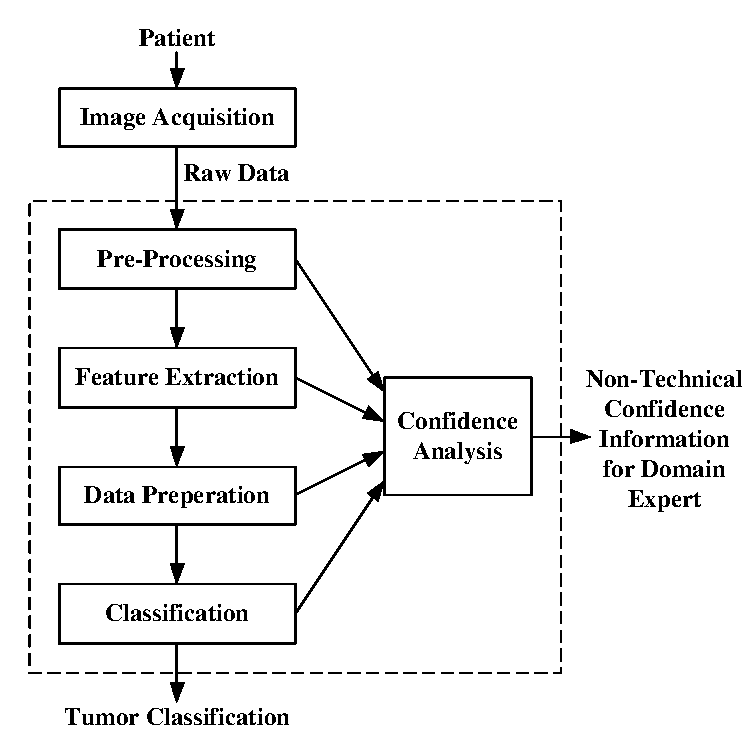
\includegraphics[width = 0.4\textwidth]{Figures/Proposed.pdf}
   \label{fig:Proposed}
   \caption{Proposed system architecture.}
\end{figure}



\section{Image Acquisition}
\label{sec:ImageAcquisition}
There are many pieces of medical equipment capable of extracting volumetric images of the human using non-invasive techniques.
Most use CT technology to build an image from 2D slices.
Here I will 




\section{Pre-processing}
\label{sec:PreProcessing}
This is how the image should be tidied before begin sent for processing.






\section{Feature Extraction}
\label{FeatureExtraction}

The possible features which can extracted.
The techniques used to extract the features.
The importance of the features.




\section{Classification}
\label{Classification}


Which classifier would perform best on this task.
Is processing heavy? Reliable?






\section{Conclusion}
\label{Conclusion}

What was good and not good.





\end{document}


